% Created 2015-04-01 Wed 21:10
\documentclass[11pt]{article}
\usepackage[utf8]{inputenc}
\usepackage[T1]{fontenc}
\usepackage{fixltx2e}
\usepackage{graphicx}
\usepackage{longtable}
\usepackage{float}
\usepackage{wrapfig}
\usepackage{rotating}
\usepackage[normalem]{ulem}
\usepackage{amsmath}
\usepackage{textcomp}
\usepackage{marvosym}
\usepackage{wasysym}
\usepackage{amssymb}
\usepackage{hyperref}
\tolerance=1000
\usepackage[utf8]{inputenc}
\usepackage[usenames,dvipsnames]{color}
\usepackage[backend=bibtex, style=numeric]{biblatex}
\usepackage{commath}
\usepackage{mathtools}
\usepackage{marginnote}
\usepackage{listings}
\usepackage{color}
\usepackage{enumerate}
\hypersetup{urlcolor=blue}
\hypersetup{colorlinks,urlcolor=blue}
\addbibresource{bibliography.bib}
\setlength{\parskip}{16pt plus 2pt minus 2pt}
\definecolor{codebg}{rgb}{0.96,0.99,0.8}
\definecolor{codestr}{rgb}{0.46,0.09,0.2}
\author{Oleg Sivokon}
\date{\textit{<2015-03-27 Fri>}}
\title{Assignment 11, Introduction to Statistics}
\hypersetup{
  pdfkeywords={Discrete Mathematics, assignment, bar chart, histogram},
  pdfsubject={First asssignment in the course Introduction to Statistics},
  pdfcreator={Emacs 25.0.50.1 (Org mode 8.2.2)}}
\begin{document}

\maketitle
\tableofcontents


\lstset{ %
  backgroundcolor=\color{codebg},
  basicstyle=\ttfamily\scriptsize,
  breakatwhitespace=false,         % sets if automatic breaks should only happen at whitespace
  breaklines=false,
  captionpos=b,                    % sets the caption-position to bottom
  commentstyle=\color{mygreen},    % comment style
  framexleftmargin=10pt,
  xleftmargin=10pt,
  framerule=0pt,
  frame=tb,                        % adds a frame around the code
  keepspaces=true,                 % keeps spaces in text, useful for keeping indentation of code (possibly needs columns=flexible)
  keywordstyle=\color{blue},       % keyword style
  showspaces=false,                % show spaces everywhere adding particular underscores; it overrides 'showstringspaces'
  showstringspaces=false,          % underline spaces within strings only
  showtabs=false,                  % show tabs within strings adding particular underscores
  stringstyle=\color{codestr},     % string literal style
  tabsize=2,                       % sets default tabsize to 2 spaces
}

\clearpage

\section{Problems}
\label{sec-1}

\subsection{Problem 1}
\label{sec-1-1}
Given the grades in an engineering faculty were as follows:

\begin{center}
\begin{tabular}{rrr}
lower & higher & graded\\
\hline
30 & 60 & 15\\
60 & 75 & 45\\
75 & 85 & 45\\
85 & 100 & 15\\
\end{tabular}
\end{center}

\begin{enumerate}
\item Present the data using a histogram.
\item Calculate mode, median, algebraic average and variance.
\item Calculate the number of students who earned at least 82 points.
\item Given the following data for the preceding year for 80 students
where the average grade was 70 and variance was 200, find the
average and the variance for two years combined.
\end{enumerate}

\subsubsection{Answer 1}
\label{sec-1-1-1}

\lstset{language=R,label=students-histogram,numbers=none}
\begin{lstlisting}
library(ggplot2)
tbl$avg <- (tbl$lower + tbl$higher) / 2
tbl$density <- 10 * tbl$graded / (tbl$higher - tbl$lower)
ggplot(tbl) + 
    geom_histogram(
        aes(x = avg, weight = density, fill = ..count..), 
        breaks = unique(append(tbl$lower, tbl$higher)),
        position = "identity", colour = "black") +
            xlab("grades")
\end{lstlisting}

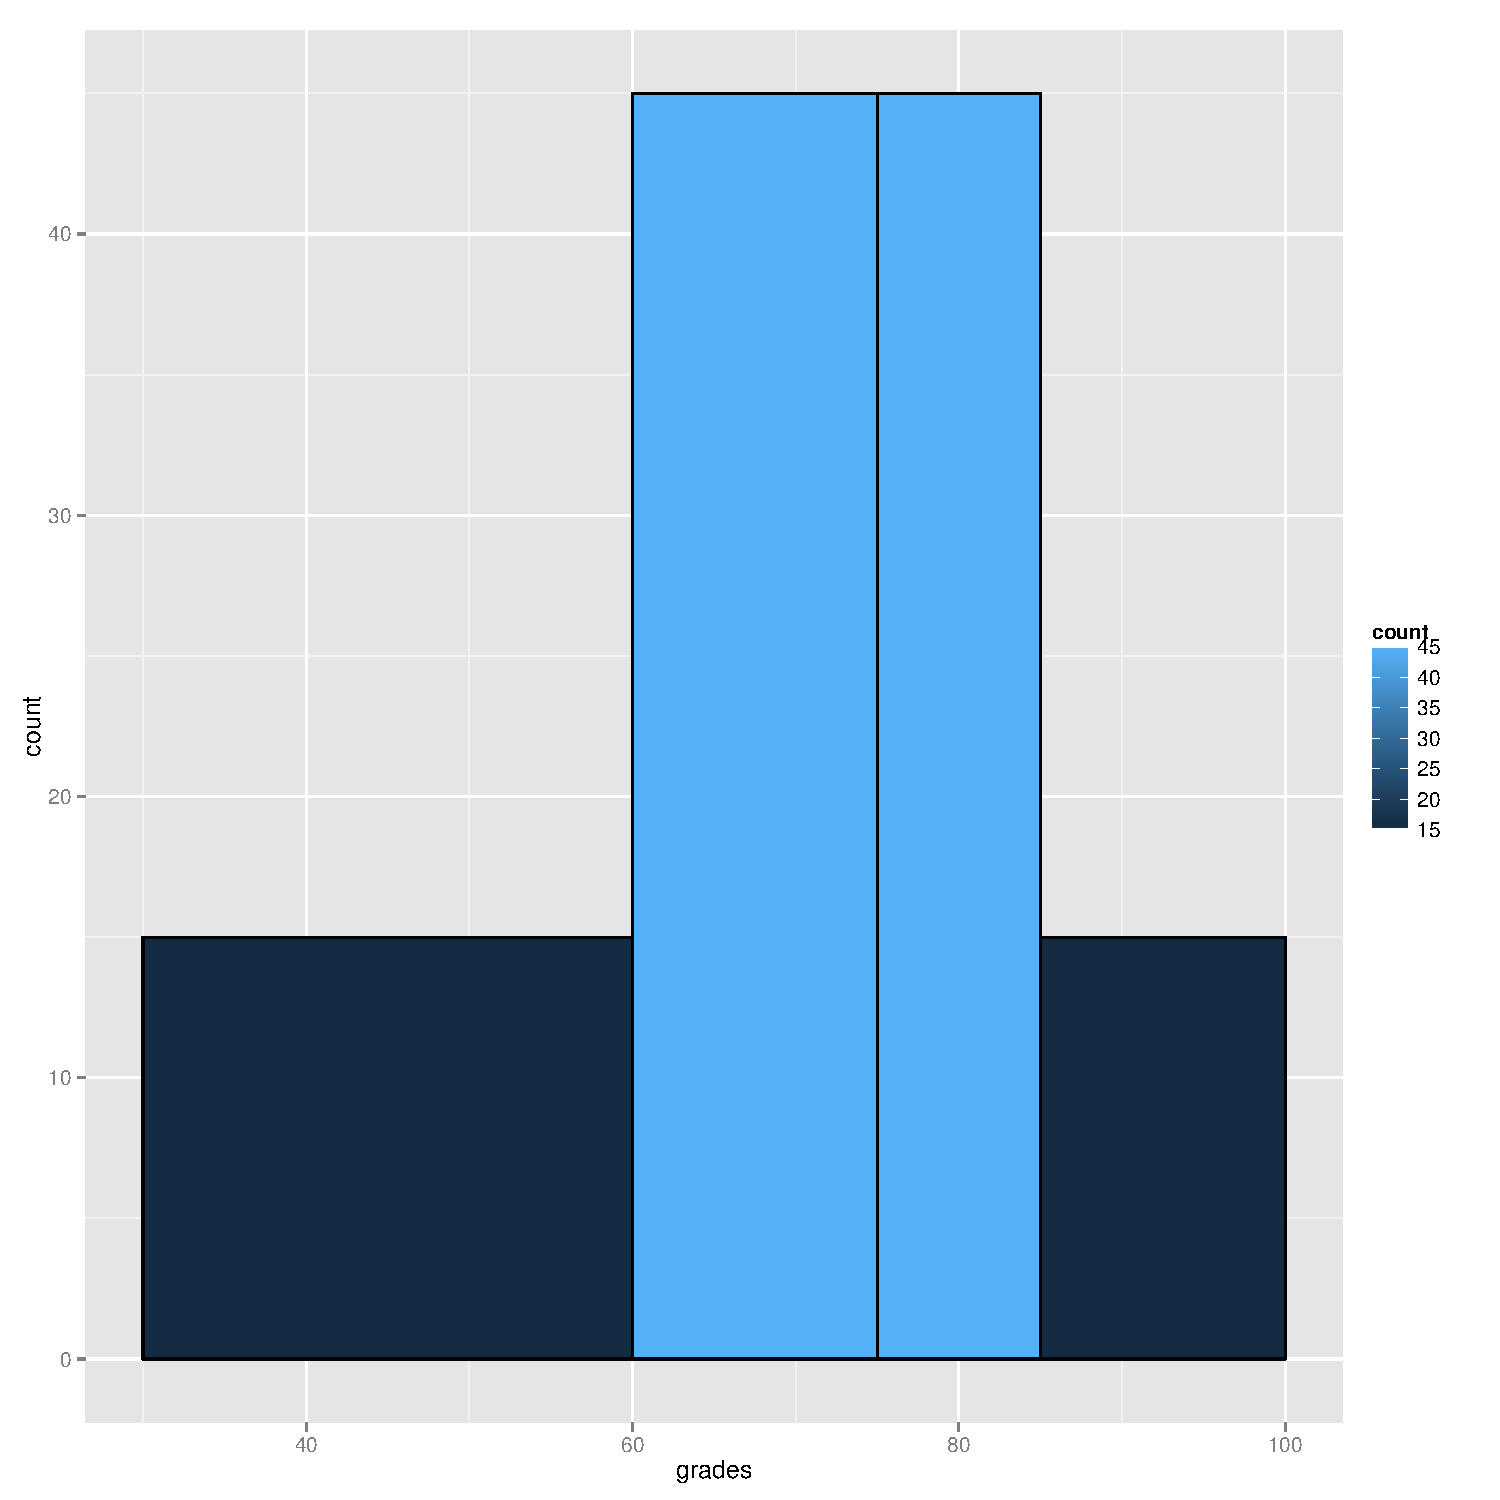
\includegraphics[width=.9\linewidth]{images/students.pdf}
\subsubsection{Answer 2}
\label{sec-1-1-2}
As easy to see from the diagram, the \textbf{mode} is in the (75, 85] range.

The \textbf{median} is the value at the 60'th studen, which is easy to see
from the table as being the 75 points.
\begin{equation*}
  \begin{aligned}
    Md &= \frac{\frac{n}{2} - F(x_{m-1})}{f(x_m)} * (L_1-L_0)+L_0 \\
    Md &= \frac{\frac{120}{2} - 60}{45} * (85 - 75) + 75 \\
    Md &= \frac{60 - 60}{45} * (85 - 75) + 75 \\
    Md &= 75
  \end{aligned}
\end{equation*}

The \textbf{average} is given by the formula:
\begin{equation*}
  \begin{aligned}
    \frac{15 * \frac{30 + 60}{2} + 45 * \frac{60 + 75}{2} +
      45 * \frac{75 + 85}{2} + 15 * \frac{85 + 100}{2}}{15 + 45 + 45 + 15} = \\
    \frac{15 * 90 + 45 * 135 + 45 * 160 + 15 * 185}{2 * 120} = \\
    \frac{17400}{240} = \\72.5
  \end{aligned}
\end{equation*}

And the \textbf{variance}:
\begin{equation*}
  \begin{aligned}
    S^2 &= \frac{\sum_1^n (x - \overline{x})^2 * f(x)}{n} \\
    S^2 &= \frac{\splitfrac{(45 - 72.5)^2 * 15 + (67.5 - 72.5)^2 * 45}
      {+ (80 - 72.5)^2 * 45 + (92.5 - 72.5)^2 * 15}}{120} \\
    S^2 &= \frac{756.25 * 15 + 25 * 45 + 56.25 * 45 + 400 * 15}{120} \\
    S^2 &= \frac{21000}{120} \\
    S^2 &= 175
  \end{aligned}
\end{equation*}
\subsubsection{Answer 3}
\label{sec-1-1-3}
Using a slightly altered formula for the median, we can calculate the 82'nd
percentile.  It is easy to see that the 82'nd percentile falls in the third
group, viz. [75, 85) interval.  Assuming values are uniformly distribute
in this interval, ${7 \over 10}$ of these are below 82 and ${3 \over 10}$
are above.  In other words, we need to take 0.3 of the 45 students in this
category, i.e. 13.5, together with 15 students who earned more points this
gives roughly 19 students.
\subsubsection{Answer 4}
\label{sec-1-1-4}
New average is just the weighted average of both averages:
$\frac{70*80+72.5*120}{80+120}=71.5$.

The total variance is calculated using
\begin{equation*}
  \begin{aligned}
    s_1 &= n(S_1 + \overline{x}^2_1) \\
    s_1 &= 120 * (175 + 72.5^2) \\
    s_1 &= 651750. \\
    s_2 &= n(S_2 + \overline{x}^2_2) \\
    s_2 &= 80 * (200 + 70^2) \\
    s_2 &= 408000.
  \end{aligned}
\end{equation*}
\begin{equation*}
  \begin{aligned}
    S^2 &= \frac{s_1 + s_2}{n_1 + n_2} - \overline{x}^2 \\
    S^2 &= \frac{651750 + 408000}{200} - 71.5^2 \\
    S^2 &= \frac{651750 + 408000}{200} - 5112.25 \\
    S^2 &= 186.5
  \end{aligned}
\end{equation*}
\subsection{Problem 2}
\label{sec-1-2}
Given the number of assignments submitted in 2009 (shown below):

\begin{center}
\begin{tabular}{rr}
assignments & students\\
\hline
0 & 11\\
1 & 18\\
2 & 28\\
3 & 22\\
4 & 15\\
5 & 16\\
\end{tabular}
\end{center}

\begin{enumerate}
\item Draw a bar chart representing the data.
\item Find mode, median, algebraic average and variance.
\item In addition to the number of assignments submitted, students
also received final grades.  Let $X$ be the number of assignments
submitted, let $Y$ be the grade the student received.  Given also that
Pearson coefficient is $r=0.75$.

\textbf{Prove or disprove:}
\begin{enumerate}
\item $Y = 0.75X + 96.25$.
\item The number of assignments submitted negatively correlates with
the final grade they received.
\end{enumerate}

\item An investigation found data on 10 more students.  5 of them didn't
submit any assignment and 5 of them submitted 5 assignments each.
Describe what will happen to each metric calculated in question 2 relying
on the previously obtained values.
\end{enumerate}

\subsubsection{Answer 5}
\label{sec-1-2-1}
\lstset{language=R,label=assignments-histogram,numbers=none}
\begin{lstlisting}
library(ggplot2)
ggplot(data = tbl, 
       aes(x = assignments, y = students, fill = assignments)) +
           geom_bar(colour = "black", stat = "identity")
\end{lstlisting}

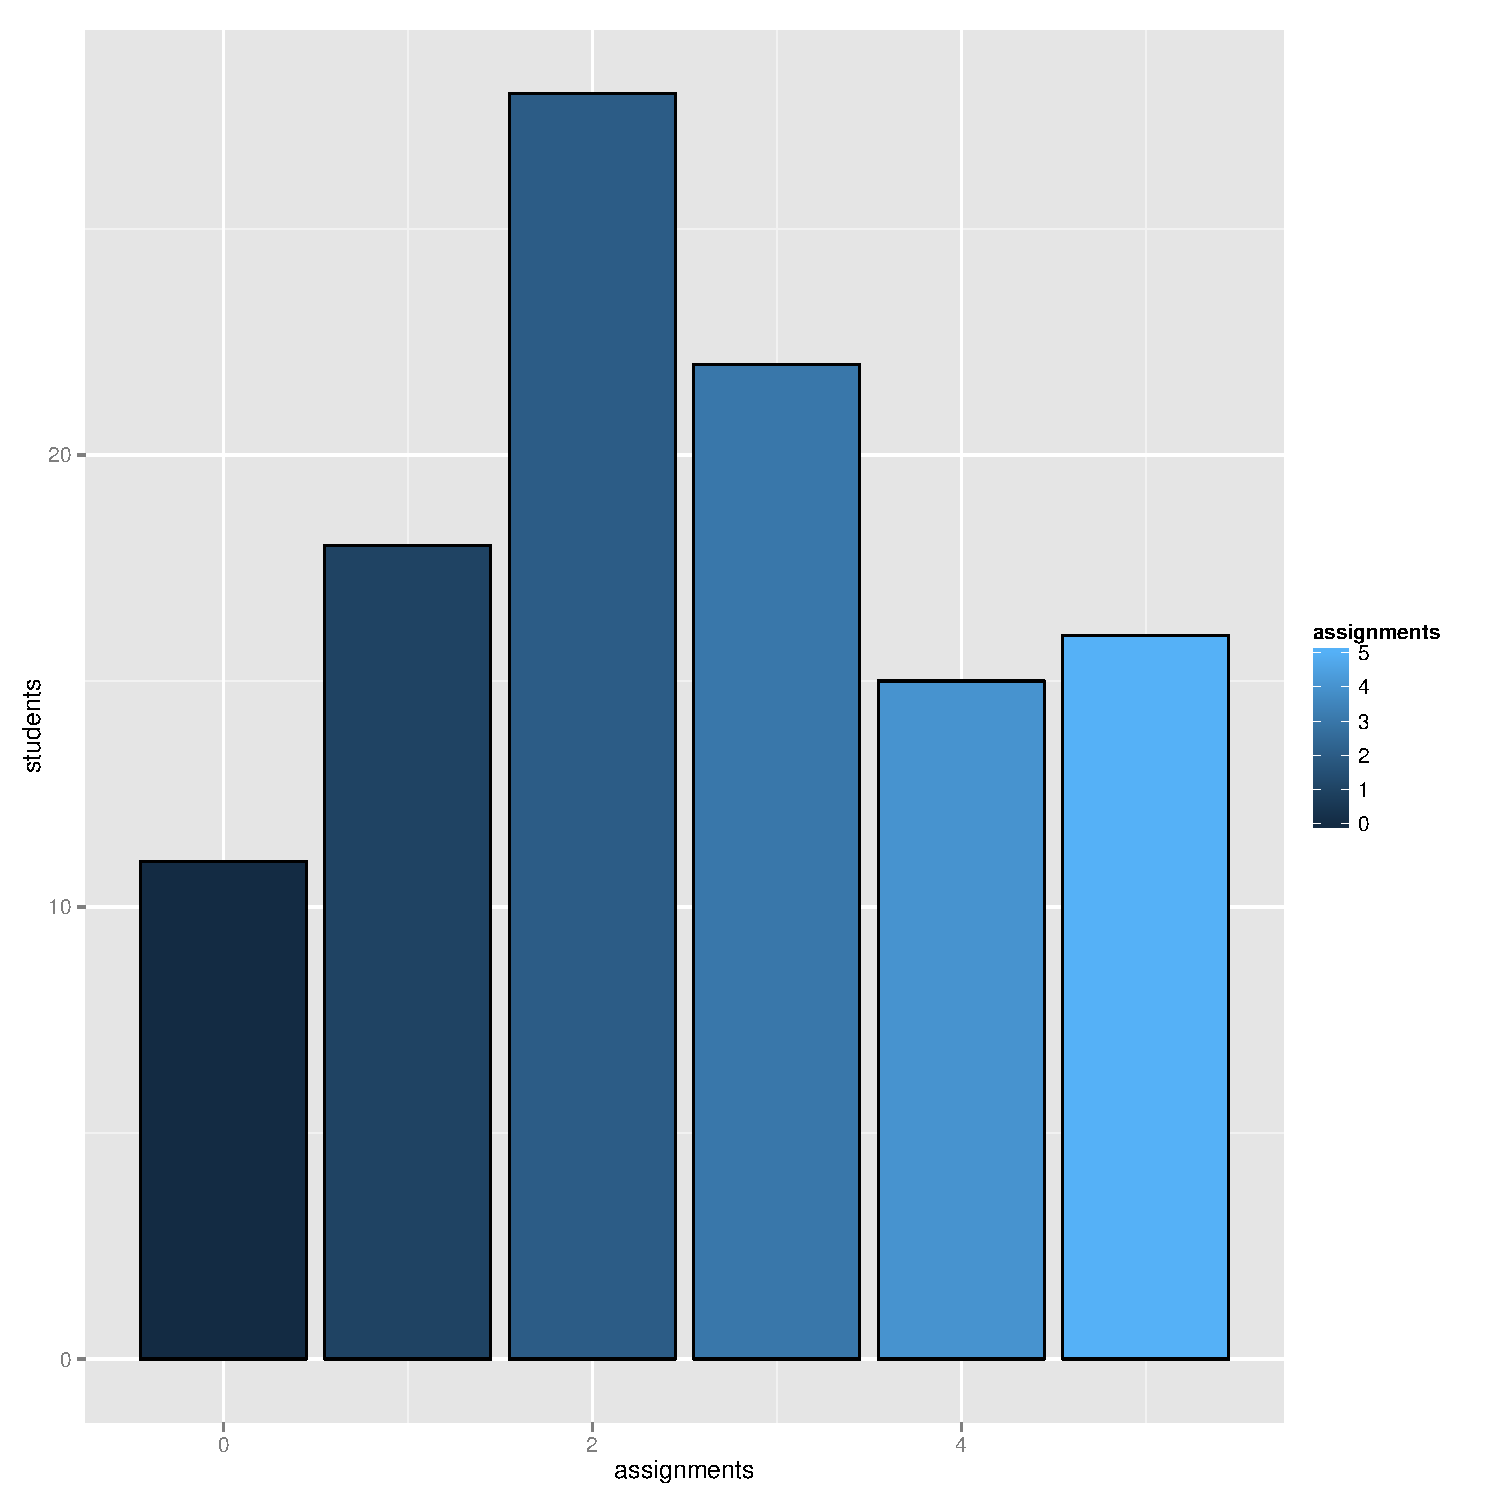
\includegraphics[width=.9\linewidth]{images/assignments.pdf}
\subsubsection{Answer 6}
\label{sec-1-2-2}
\textbf{Mode} for the assignments data is 2, i.e. most of the students submitted
only two assignments.

\textbf{Median} is $2+(3-2)/2=2.5$ (because there is an even number of bins).

Weighted \textbf{average} can be obtained using
$\frac{0*11+1*18+2*28+3*22+4*15+5*16}{110}=\frac{280}{110}=2.45(45)$.

\textbf{Variance} can be obtained using:
\begin{equation*}
  \begin{aligned}
    S^2 &= \frac{(0 * 11)^2 + (1 * 18)^2 + (2 * 28)^2 +
      (3 * 22)^2 + (4 * 15)^2 + (5 * 16)^2}{110} - 2.45^2 \\
    S^2 &= \frac{17816}{110} - 6.0025 \\
    S^2 &= 161.963636364 \\
    S^2 &\simeq 162
  \end{aligned}
\end{equation*}

\subsubsection{Answer 7}
\label{sec-1-2-3}
While it seems appealing, it isn't really possible to have a determination
coefficient predict the value of another variable with absolute certainity
unless the coefficient is equal to one.  Thus $Y = 0.75X + 96.25$ is at best
a lucky coincidence.

Positive coefficient means that there exists positive correlation between
two variables.  In particular, it means that roughly in three fourth of all
cases the number of assignments submited perfectly predicted the final grade.
So the claim is obviously false.
\subsubsection{Answer 8}
\label{sec-1-2-4}
After adding ten more observations the \textbf{mode} will not change as the
observations fall into the bins which aren't as dense as the most dense one,
i.e. the first bin will contain 11+5=16 students
\emph{(fewer than 28 of the densest bin)} and 6+5=11 in the last bin.

The \textbf{median} will not change either because we are adding observations to
the outermost bins in an equal measure.

The \textbf{average} will almost not change because the added observations will
``cancel out'', however, it will shift very slightly towards the upper
end, since we increased the relative weight of the bin of those who
submitted the most assignments.

Since \textbf{variance} is affected by the mean, it is hard to tell without
doing full recalculation whether it will or will not change.  However,
since we added more borderline observations, which are most likely to
be far away from the mean, we'd expect the variance to grow.
\subsection{Problem 3}
\label{sec-1-3}
Given the histogram below:


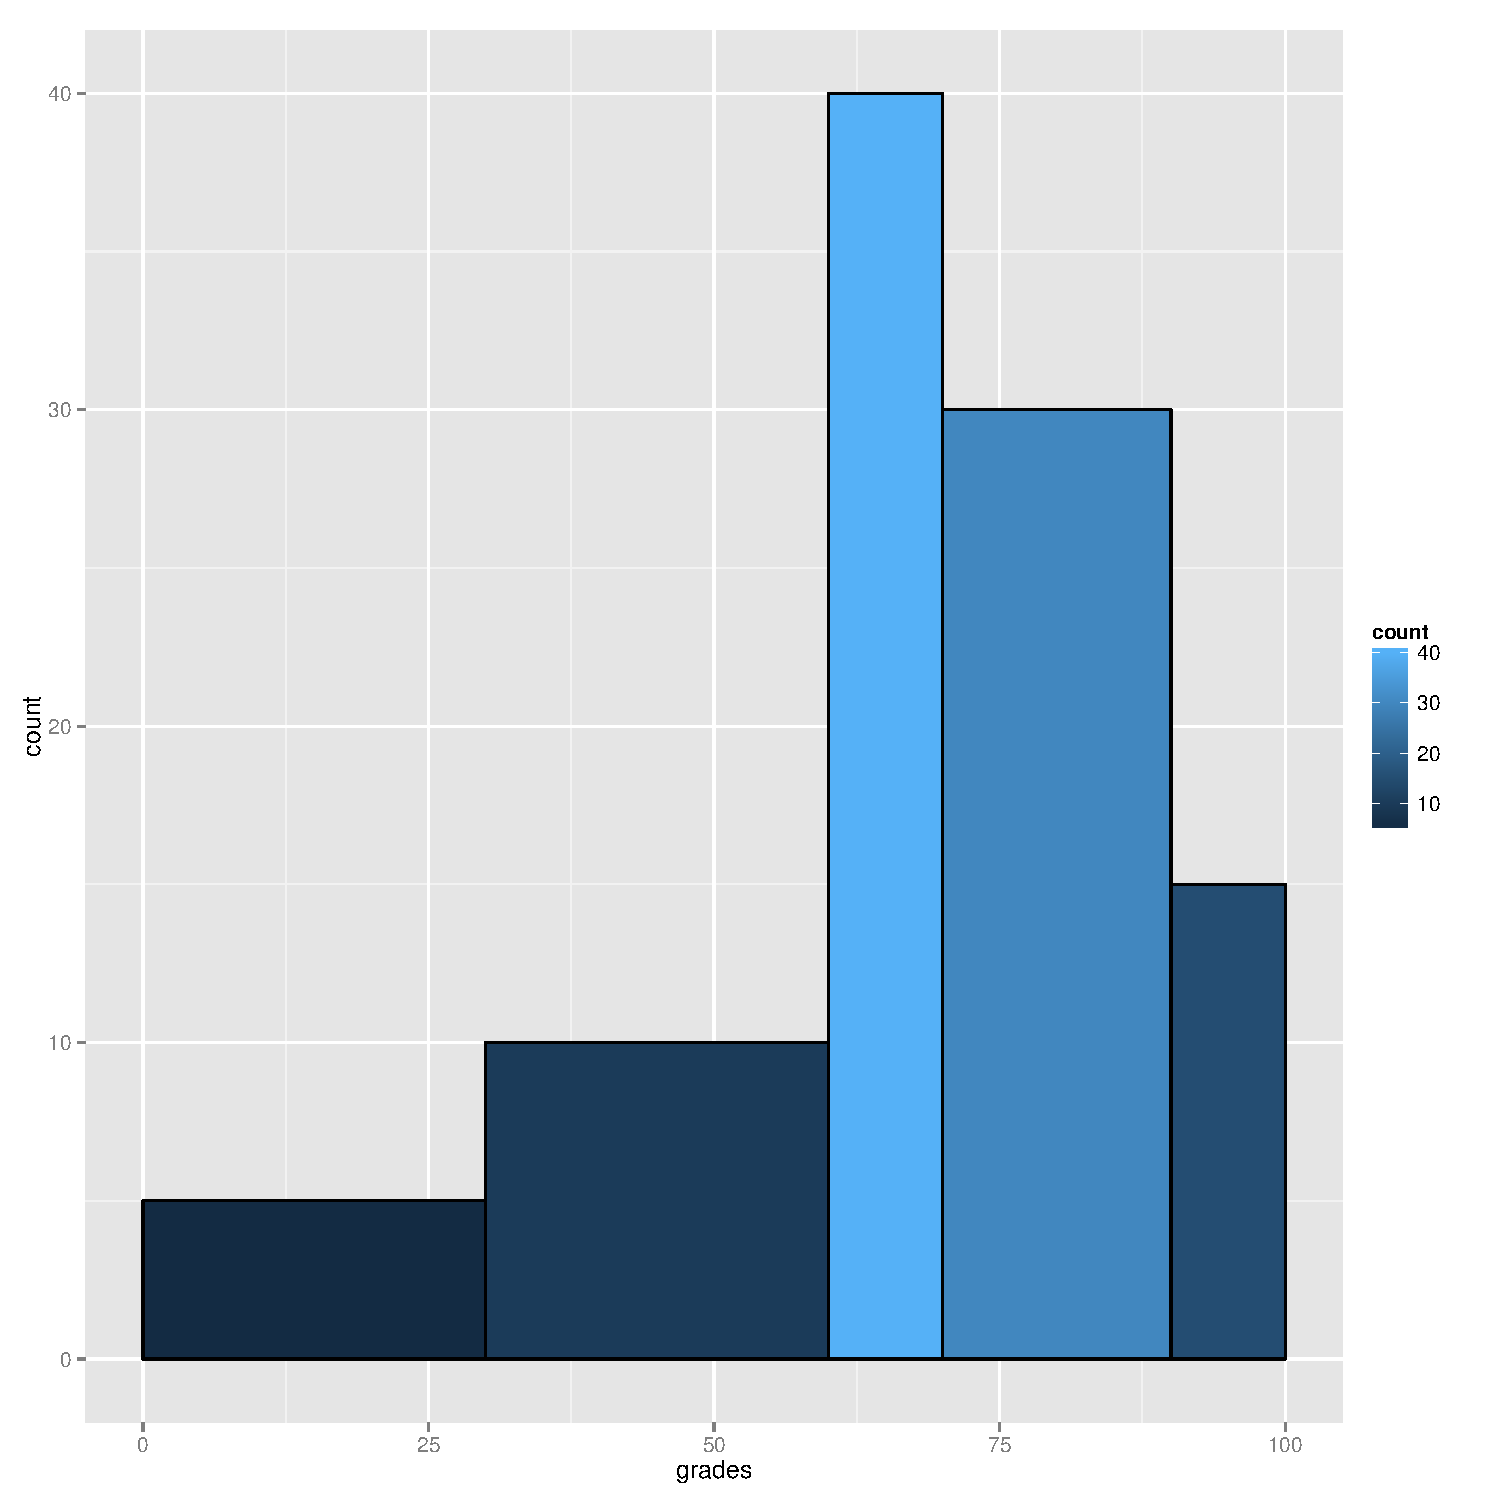
\includegraphics[width=.9\linewidth]{images/exam.pdf}

\begin{enumerate}
\item Write the spread of the diagram.
\item Calculate the mode, median, average and standard deviation.
\item Students Paz, Or and Nadav received the following grades:
\begin{description}
\item[{Paz}] Has standard score of 0.75.
\item[{Or}] Was awarded 75 points.
\item[{Nadav}] Is in the 80'th percentile.
\end{description}
Rank Paz, Or and Nadav according to their grades from 
lowest to highest.
\item After the exam took place, the grader decided to award additional
ten points to every student s.t. the resulting grade will not be greater
than 100.

Prove or disprove:
\begin{enumerate}
\item The new average is 72.5.
\item Standard deviation grew as the result of the change.
\end{enumerate}
\end{enumerate}

\subsubsection{Answer 9}
\label{sec-1-3-1}
As can be infered from the diagram, the grades were divides as shown below:

\begin{center}
\begin{tabular}{rrrrr}
low & high & students & F(students) & f(students)\\
\hline
0 & 30 & 15 & 15 & 15\\
30 & 60 & 30 & 45 & 45\\
60 & 70 & 40 & 85 & 65\\
70 & 90 & 60 & 145 & 80\\
90 & 100 & 15 & 160 & 95\\
\end{tabular}
\end{center}
\subsubsection{Answer 10}
\label{sec-1-3-2}
The \textbf{mode}, as can be seen in the diagram is 40.

The \textbf{median} is in the middle of the third group (at position 80), which
gives, using the formula:
\begin{equation*}
  \begin{aligned}
    Md &= \frac{\frac{n}{2} - F(x_{m-1})}{f(x_m)} * (L_1-L_0)+L_0 \\
    Md &= \frac{\frac{160}{2} - 45}{65} * (70 - 60) + 60 \\
    Md &= \frac{80 - 45}{65} * 10 + 75 \\
    Md &= \frac{70}{13} + 75 \\
    Md &= 80.3846153846.
  \end{aligned}
\end{equation*}

The \textbf{average} can be obtained via $\frac{15*15+30*45+40*65+60*80+15*95}{160}=65$.

The \textbf{standard deviation} can be obtained via:
\begin{equation*}
  \begin{aligned}
    \sigma &= \sqrt{\frac{\sum_{i=1}^n (x-\overline{x})^2}{n}} \\
    \sigma &= \sqrt{\frac{\splitfrac{15 * (15 - 65)^2 + 30 * (45 - 65)^2}
        {+ 40 * (65 - 65)^2 + 60 * (80 - 65)^2 + 15 * (95 - 65)^2}}{160}} \\
    \sigma &= \sqrt{\frac{76500}{160}} \\
    \sigma &= 21.8660696057.
  \end{aligned}
\end{equation*}
\subsubsection{Answer 11}
\label{sec-1-3-3}
First, we'll calculate \textbf{Paz}'s grade.  Given the formula:
$Z_x=\frac{x-\overline{x}}{S_x}$ obtains $x=Z_xS_x + \overline{x}$,
substituting known values gives $x=0.75 * 25 + 80.4 \simeq 98$.

Now, let's find \textbf{Nadav}'s grade.  Using the percentile formula:
\begin{equation*}
  \begin{aligned}
    C_k &= \frac{\frac{nk}{100} - F(x_{m-1})}{n}(L_1 - L_0) + L_0 \\
    C_k &= \frac{\frac{160*82}{100} - 85}{80}(90 - 70) + 70 \\
    C_k &= \frac{1.6*82 - 85}{80} * 20 + 70 \\
    C_k &= \frac{46.2}{4} + 70 \\
    C_k &= 81.55.
  \end{aligned}
\end{equation*}

In conclusion, it looks like Or received the lowest grade (75), right
after him was Nadav, with 82 points, and Paz was a clear leader,
receiving a whooping 98 points.
\subsubsection{Answer 12}
\label{sec-1-3-4}
One way to look at what has happened is to notice that each group of
students had to lose a number of students due to them receiving higher
grades (except for the last group), and each group would gain some
students (those transfered from the one below it in the rating),
except, again, for the first one.  Assuming uniform distributin inside
the bins, we can derive a formulat to calculate the number of students
transfered: $\frac{L_1 - 10}{L_1 - L_2}f(x)$, where $L_1$ is the lower
bound on the group and $L_2$ is the higher bound.  The table below
provides a complete calculation:

\begin{center}
\begin{tabular}{rrrrrrr}
low & high & students & out & in & new & avg\\
\hline
0 & 30 & 15 & 5 & 0 & 10 & 15\\
30 & 60 & 30 & 10 & 5 & 25 & 45\\
60 & 70 & 40 & 40 & 10 & 10 & 65\\
70 & 90 & 60 & 30 & 40 & 70 & 80\\
90 & 100 & 15 & 0 & 30 & 45 & 95\\
\end{tabular}
\end{center}

Which gives us the new average:
$\frac{10*15+25*45+10*65+70*80+45*95}{160}=\frac{11800}{160}=73.75$.
Thus the answer it, no, new average is not 72.75 (but close).

Without recalculating the standard deviation, it is reasonable to
assume that the margins of the distribution narrowed, but it doesn't
hurt to calculate it, which gives:
\begin{equation*}
  \begin{aligned}
    \sigma &= \sqrt{\frac{\splitfrac{10 * (15 - 73.75)^2 + 25 * (45 - 73.75)^2}
          {+ 10 * (65 - 73.75)^2 + 70 * (80 - 73.75)^2 + 45 * (95 - 73.75)^2}}{160}} \\
    \sigma &= \sqrt{\frac{79000}{160}} \\
    \sigma &= 22.2204860433.
  \end{aligned}
\end{equation*}

Which is proves our initial assumption to be wrong, indeed the standard
deviation grew as a result of this change.
\subsection{Problem 4}
\label{sec-1-4}
Given the table of overdue assignments:

\begin{center}
\begin{tabular}{rr}
days & students\\
\hline
0 & 18\\
1 & 10\\
2 & 4\\
3 & 5\\
4 & 2\\
5 & 1\\
\end{tabular}
\end{center}

\begin{enumerate}
\item Present the data using a bar chart.
\item Find mode, median, average and variance.
\item The professor decided to deduce 5 points for each day past the submission
deadline.  Provided the students could've been awarded at most 100 points
before deduction, calculate the maximum average and maximum variance after
deduction.
\item The professor forgot to add five more records of students who submitted
their assignments even later than the rest.  After these data are added,
what will happen to the statistics calculated in (2)?
\end{enumerate}

\subsubsection{Answer 13}
\label{sec-1-4-1}
\lstset{language=R,label=overdue-barchart,numbers=none}
\begin{lstlisting}
library(ggplot2)
ggplot(data = tbl, 
       aes(x = days, y = students, fill = days)) +
           geom_bar(colour = "black", stat = "identity")
\end{lstlisting}

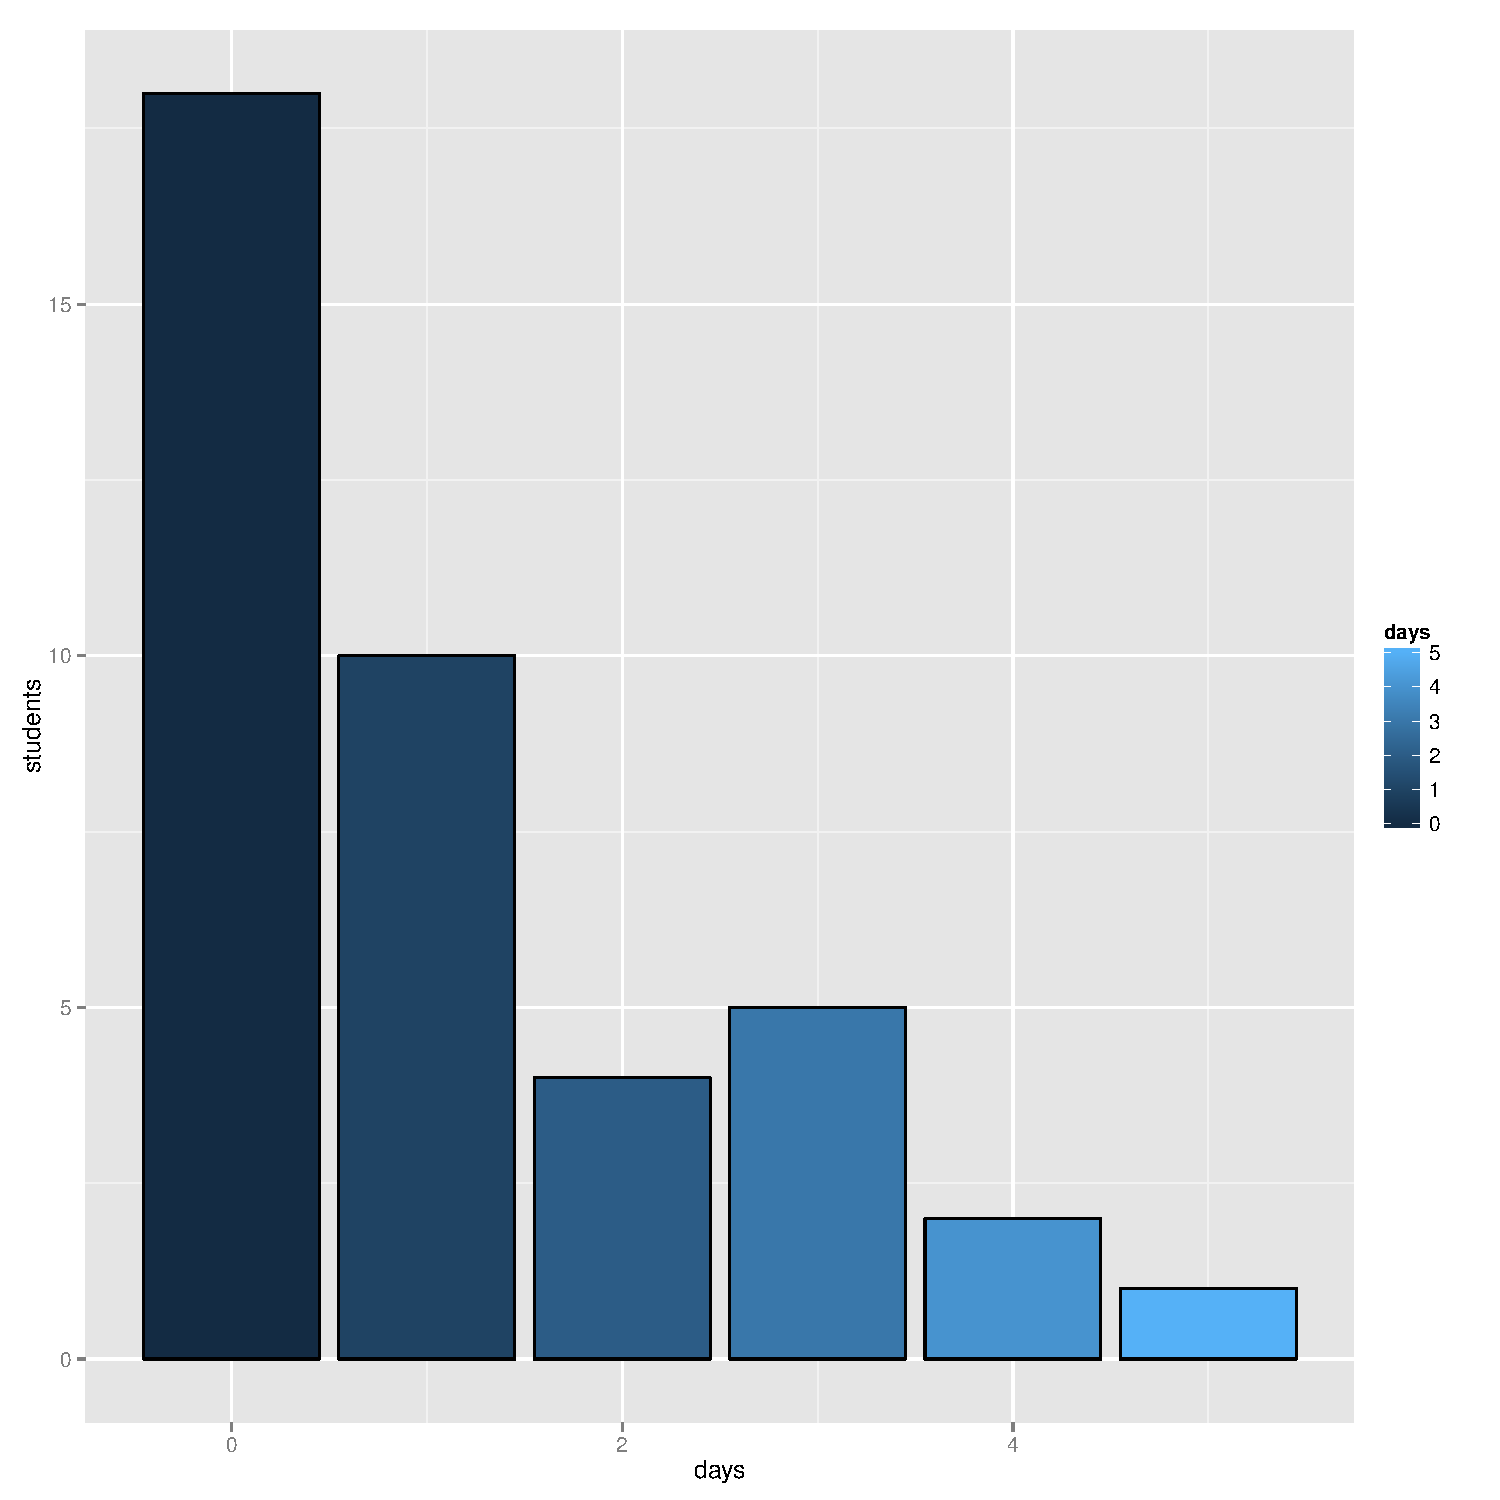
\includegraphics[width=.9\linewidth]{images/overdue.pdf}
\subsubsection{Answer 14}
\label{sec-1-4-2}
As is easy to see from the diagram, the \textbf{mode} is 0 (i.e. most students
submitted their assignments on time).

The \textbf{median} is is betwen the 20'th and the 21'st students (since there are
in total 40 observations), and it is 1.

The \textbf{average} is $\frac{18*0+10*1+4*3+5*3+2*4+1*5}{40}=1.25$.

The \textbf{variance} is thus:
\begin{equation*}
  \frac{\splitfrac{(18 * (0 - 1.25)^2 + 10 * (1 - 1.25)^2 + 4 * (3 - 1.25)^2}
    {+ 5 * (3 - 1.25)^2 + 2 * (4 - 1.25)^2 + 1 * (5 - 1.25)^2}}{40} = 2.1375.
\end{equation*}
\subsubsection{Answer 15}
\label{sec-1-4-3}
It is easy to calculate the points deduced as a weighted sum of days, weighted
by students, i.e. $5*(0*18+1*10+2*4+3*5+4*2+3*1)=220$, while total number of
points before deduction is $40*100=4000$, thus $\frac{4000-220}{40}=94.5$
would be the \textbf{average} after deduction.

Using the average, we can now find \textbf{variance} 

\begin{equation*}
  \begin{aligned}
    \frac{\splitfrac{18 * (0 * 100)^2 + 1 * (10 * 95)^2 + 2 * (4 * 90)^2}
      {+ 3 * (5 * 85)^2 + 4 * (2 * 80)^2 + 3 * (1 * 75)^2}}{40} - 94.5^2 = \\
    \frac{1822850}{40} - 8930.25 = 36641.
  \end{aligned}
\end{equation*}
\subsubsection{Answer 16}
\label{sec-1-4-4}
After more observations are added, the \textbf{mode} will not change (it will still
be the most common case that the most students submitted their assignments on
time).  The \textbf{median} will not change either, however now the median student
will be the 23'rd one, but that student is still the one who submitted the
assignment one day overdue.  The average will slightly increase (since we
added more students who are in a category far away from the old average).
Finally, the variance will likely increase too, since we are adding observations
which are far away from the average.
% Emacs 25.0.50.1 (Org mode 8.2.2)
\end{document}